\chapter{Lattice Elements}
\label{s:gui.lat}

The GUI provides the ability to view and edit the elements of a lattice through the lattice table window and through the element browser.

%-----------------------------------------------------------------
\section{Viewing the Lattice}
\label{s:gui.lat.table}

\begin{figure}
\centering
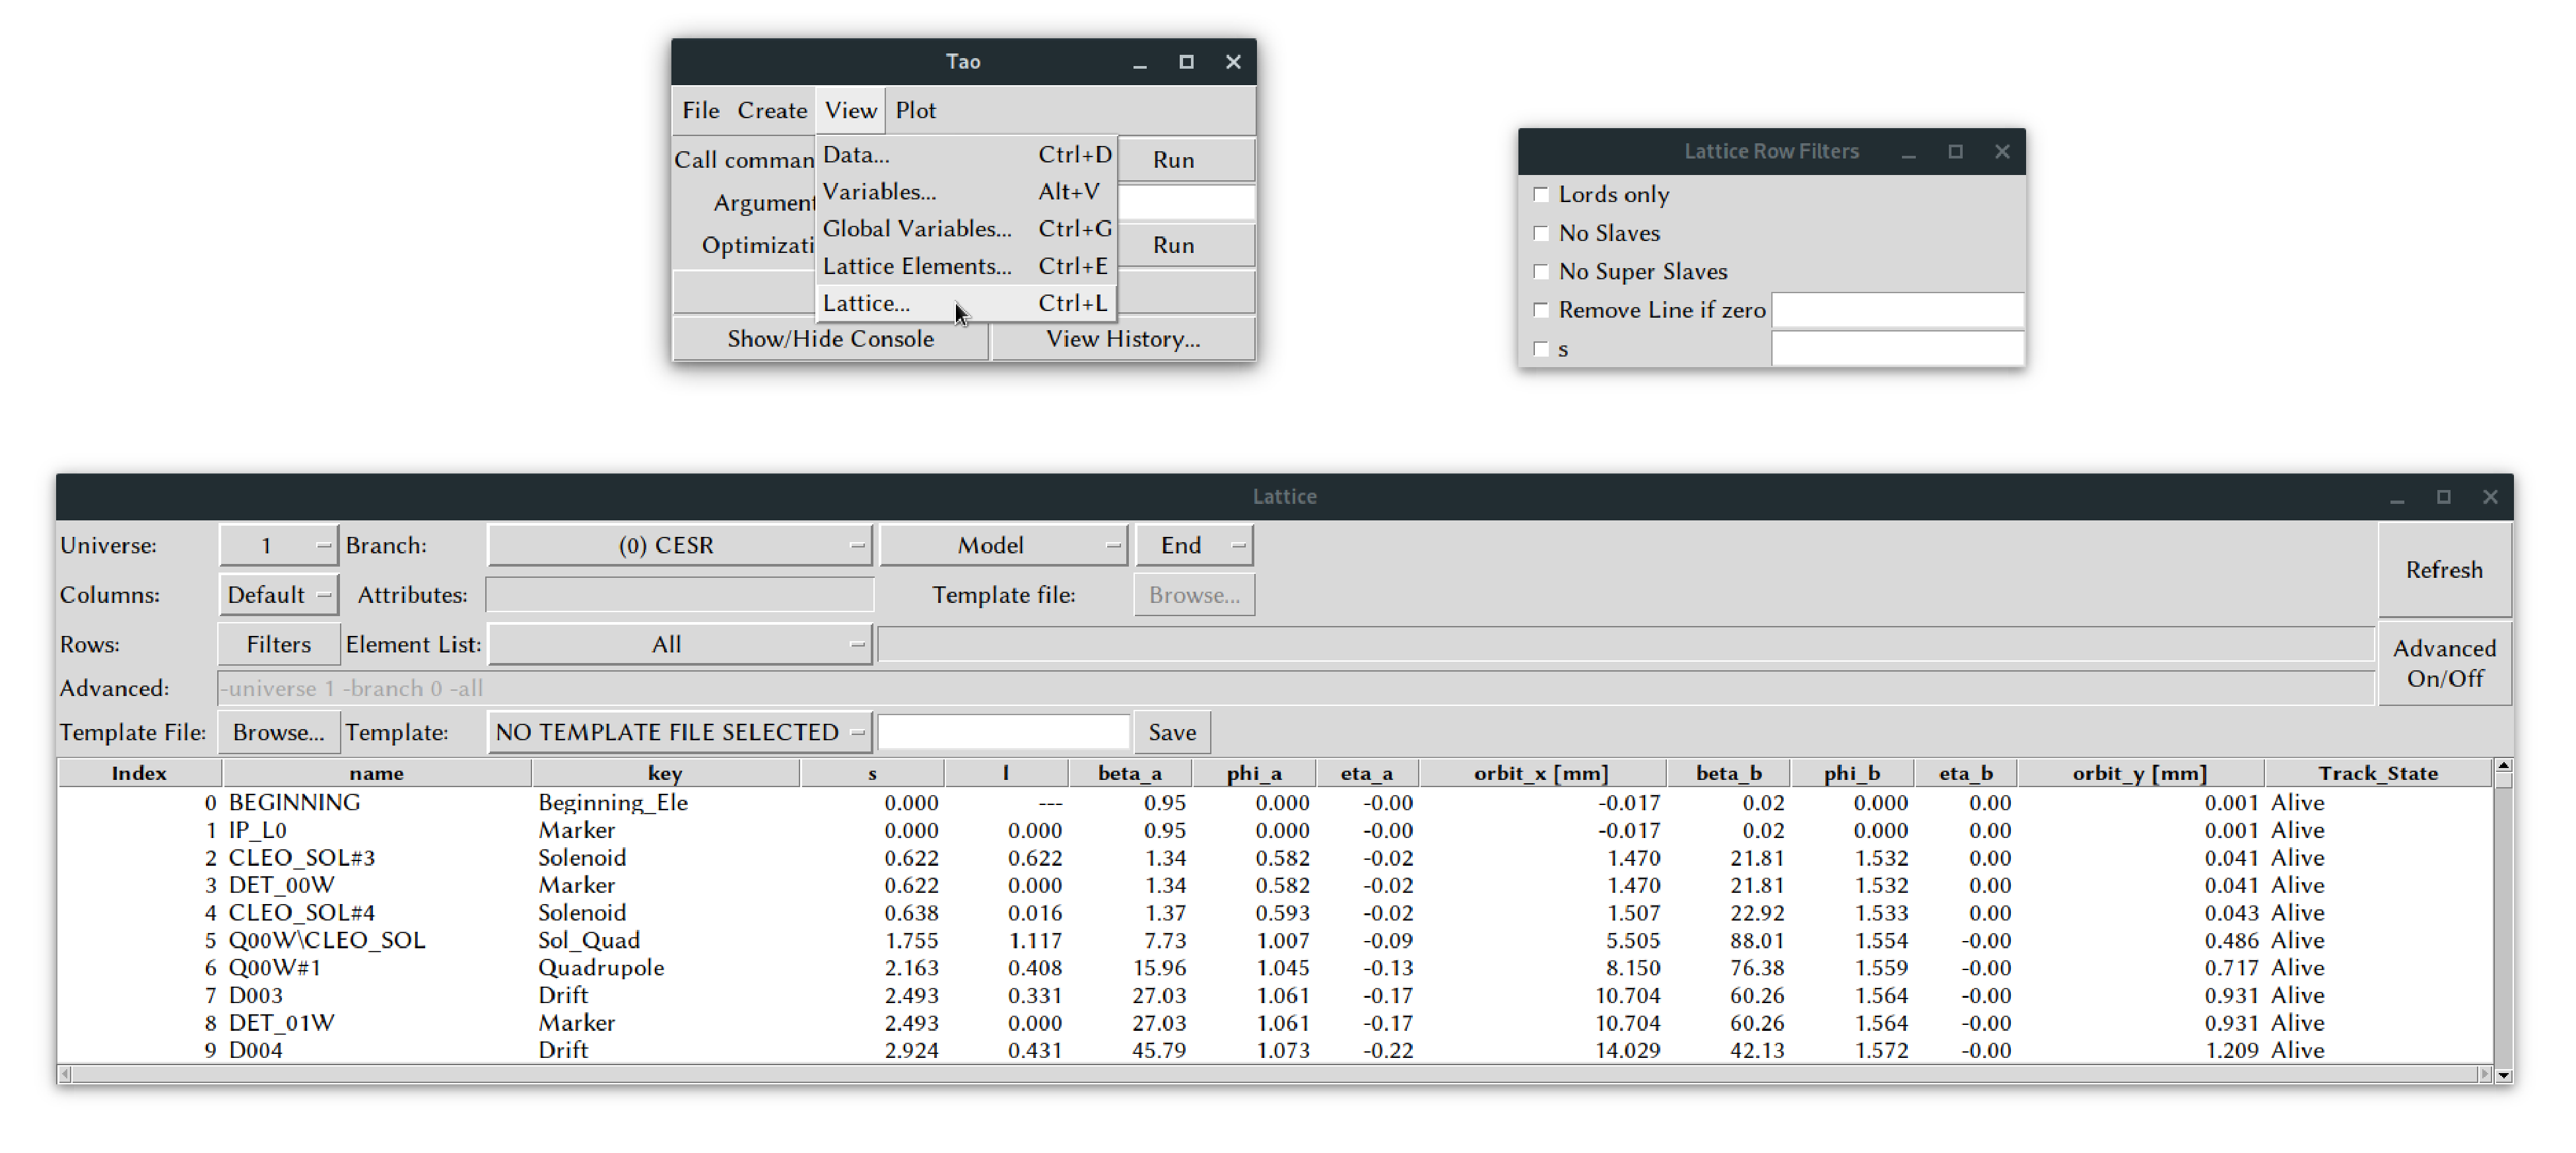
\includegraphics[width=12cm]{figures/lat_table.pdf}
\caption[The lattice table window.]{The lattice table window.
Top left: accessing the lattice table window from the root window.
Bottom: The lattice table window in its default state.
Top right: the row filter window for the lattice table window.}
\label{fig:gui.lat.table}
\end{figure}

The primary window for viewing the lattice is the lattice table window, as shown in Figure \ref{fig:gui.lat.table}.
The top portion of the window allows the lattice table to be manipulated, while the bottom portion of the window shows the requested lattice elements and properties.

The first row of settings allows the user to specify the universe and branch of interest, as well as whether base, model, or design parameters should be used, and whether they should be evaluated at the beginning, middle, or end of each element.

The next row allows the user to control what information will be shown in the columns of the table.
Some common presets are available in the drop down menu, but attributes can also be listed manually in the "Attributes" text box.
A lattice template file can also be loaded to determine the column settings (TODO: reference appropriate section in Tao manual).

The next row allows the user to specify which elements will appear in the table.
Clicking on the "Filters" button will open the lattice row filter window (top right in Figure \ref{fig:gui.lat.table}).
The first three settings in this window allow the user to filter in/out the lord and slave elements as desired.
The fourth setting in this window, "Remove line if zero", will filter out any rows that have $0$ in the specified column number.
The final setting in this window allows the user to specify a particular range of s values that elements must have.
Only elements with s within the specified range will be displayed.
The elements to be displayed in the table can also be specified with the "Element List" in the lattice table window.
The user can choose to show all elements, only tracking elements, or a custom list of elements.

The "Advanced" row allows the user to directly set the switches that determine the lattice table, as described in Section (TODO: reference \texttt{show lat} portion of Tao manual).
This box can be toggled on and off with the "Advanced on/off" button to the right of the window.

The final row allows the user to load and save a lattice template file as described in Section \ref{s:gui.lat.templates}.
Loading a template file will populate the template drop-down menu with the defined templates.
The user can also save the current lattice table settings by entering a template name and clicking the "Save button", which will add the new template to the currently open template file.

Once the settings have been adjusted, clicking the "Refresh" button will populate the lattice table according to the specified settings.
The table is scollable, and lists the lord elements at the end of the table if there are any to show.
Double clicking on a row of the table will open an element window for the selected lattice element (see Section \ref{s:gui.lat.elements}).

Figure \ref{fig:gui.lat.table.example} shows an example of the lattice table's capabilities.
\begin{figure}
\centering
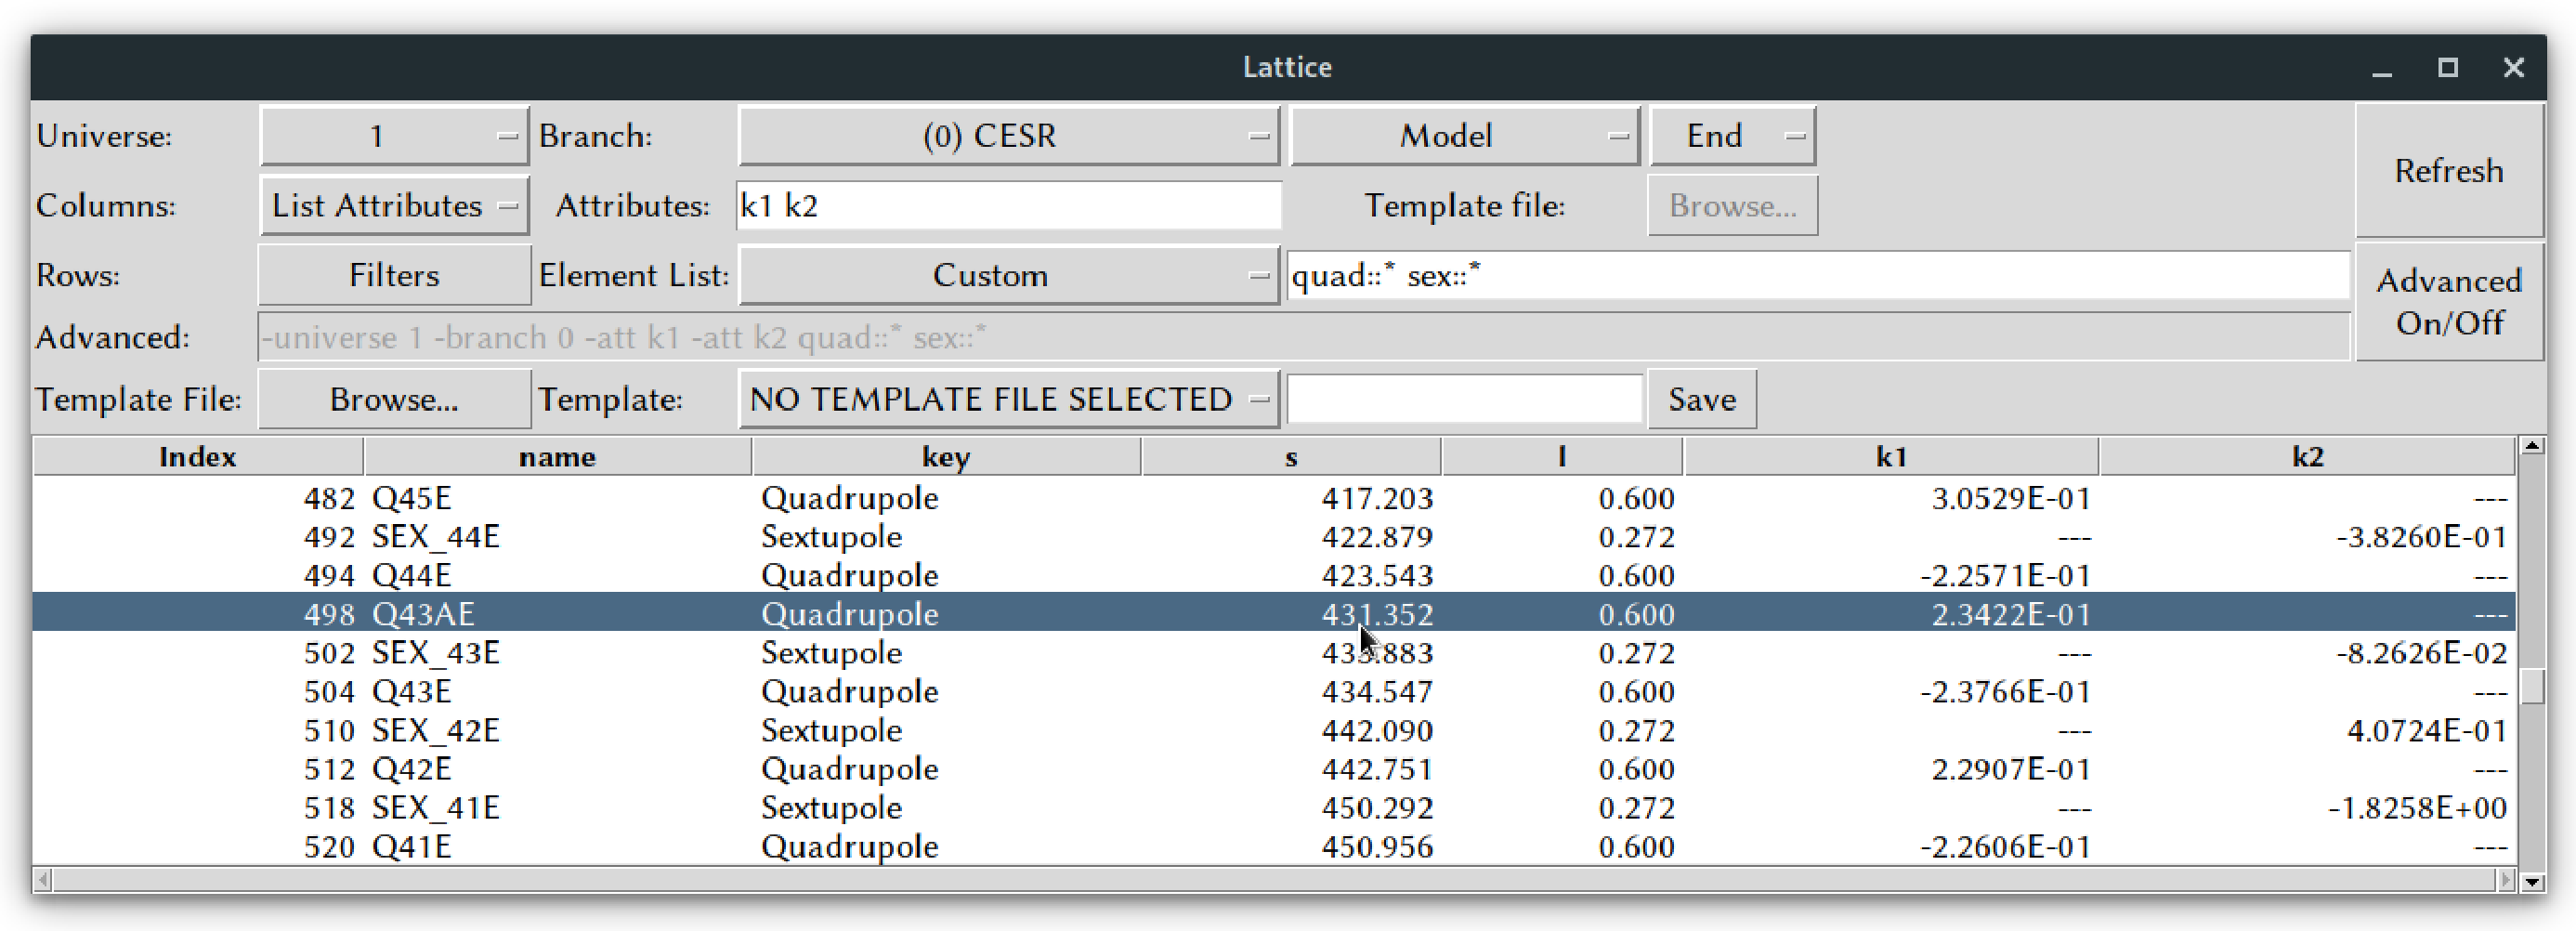
\includegraphics[width=12cm]{figures/lat_table_example.pdf}
\caption[An example of the lattice table in use.]{An example of the lattice table in use.
Here, the table displays all quadrupoles and sextupoles in the lattice, with their k1 and k2 attributes.}
\label{fig:gui.lat.table.example}
\end{figure}
In this example, the user has selected the quadrupole and sextupole elements to be displayed, and has set the k1 and k2 attributes of each element to be shown.

%-----------------------------------------------------------------
\section{Lattice Templates}
\label{s:gui.lat.templates}

You can save your settings from the lattice table window in a template file, which can then be loaded and added to from within the gui.
The file can be named anything, and the formatting is as follows:
Lines starting with \# are considered comments and ignored.
Lines starting with "name:" are interpreted as a name for the settings listed in the line directly below
All other lines are interpreted as switches, as would be used with the show lattice command in Tao (see the tao manual for more info).
All switches for a given template should be on one line.

Example:
\begin{example}
#MY TEMPLATE FILE
name:template 1
-orbit -spin -tracking_elements
name:template 2
-lords q*
name: another template
-floor_coords -s 10:20
-radiation_integrals -all
\end{example}

This template file defines four templates: "template 1", "template 2", "another template", and an unnamed template (which has the switches -radiation_integrals -all).  Named templates are displayed by name in the gui, while unnamed templates are simply displayed by what switches they specify.

%-----------------------------------------------------------------
\section{Viewing a Lattice Element}
\label{s:gui.lat.elements}

Individual lattice elements can be viewed and editted with the lattice element window as shown in Figure \ref{fig:gui.lat.element.1}.
\begin{figure}
\centering
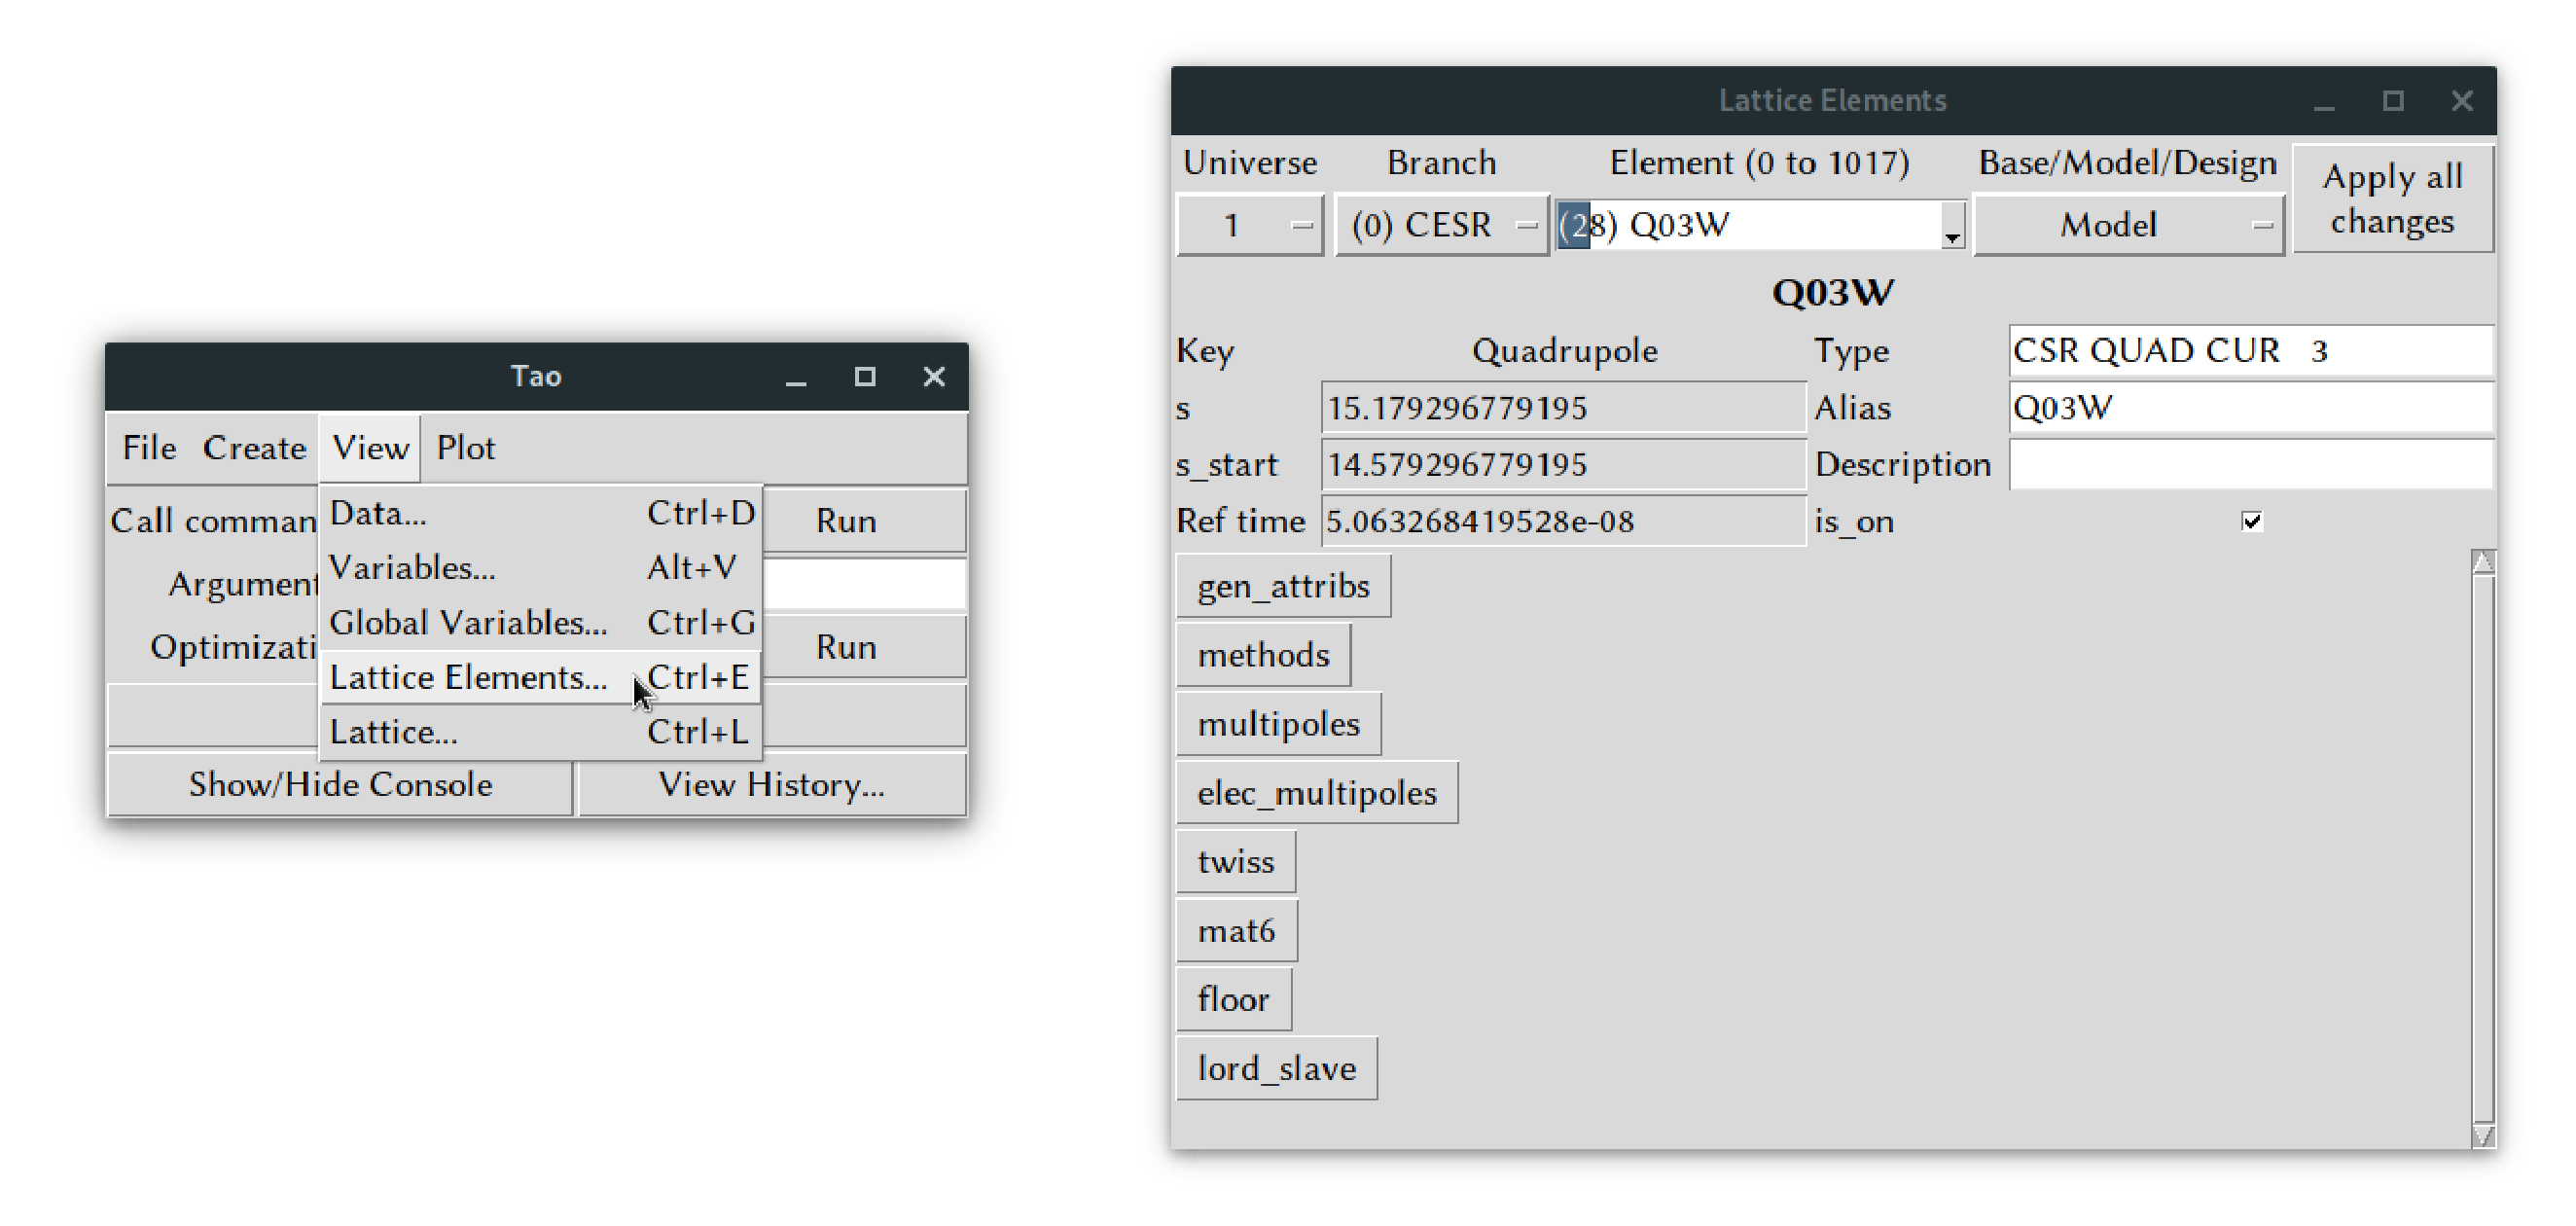
\includegraphics[width=12cm]{figures/lat_element_1.pdf}
\caption[Accessing the lattice element window.]{Accessing the lattice element window.
Here, element Q03W is displayed, with all of its sub-sections collapsed.}
\label{fig:gui.lat.element.1}
\end{figure}
The drop down menus at the top of the window allow the user to select the element to be displayed, as well as whether base, model, or design attributes should be shown.
The next section of the window displays some basic information about the element, some of which can be editted by the user.

The rest of the window is devoted to showing and editting the properties of the selected element.
These properties are divided into sections that can be expanded and collapsed by clicking on the section name.
An example of some of these sections is shown in Figure \ref{fig:gui.lat.element.2}.
\begin{figure}
\centering
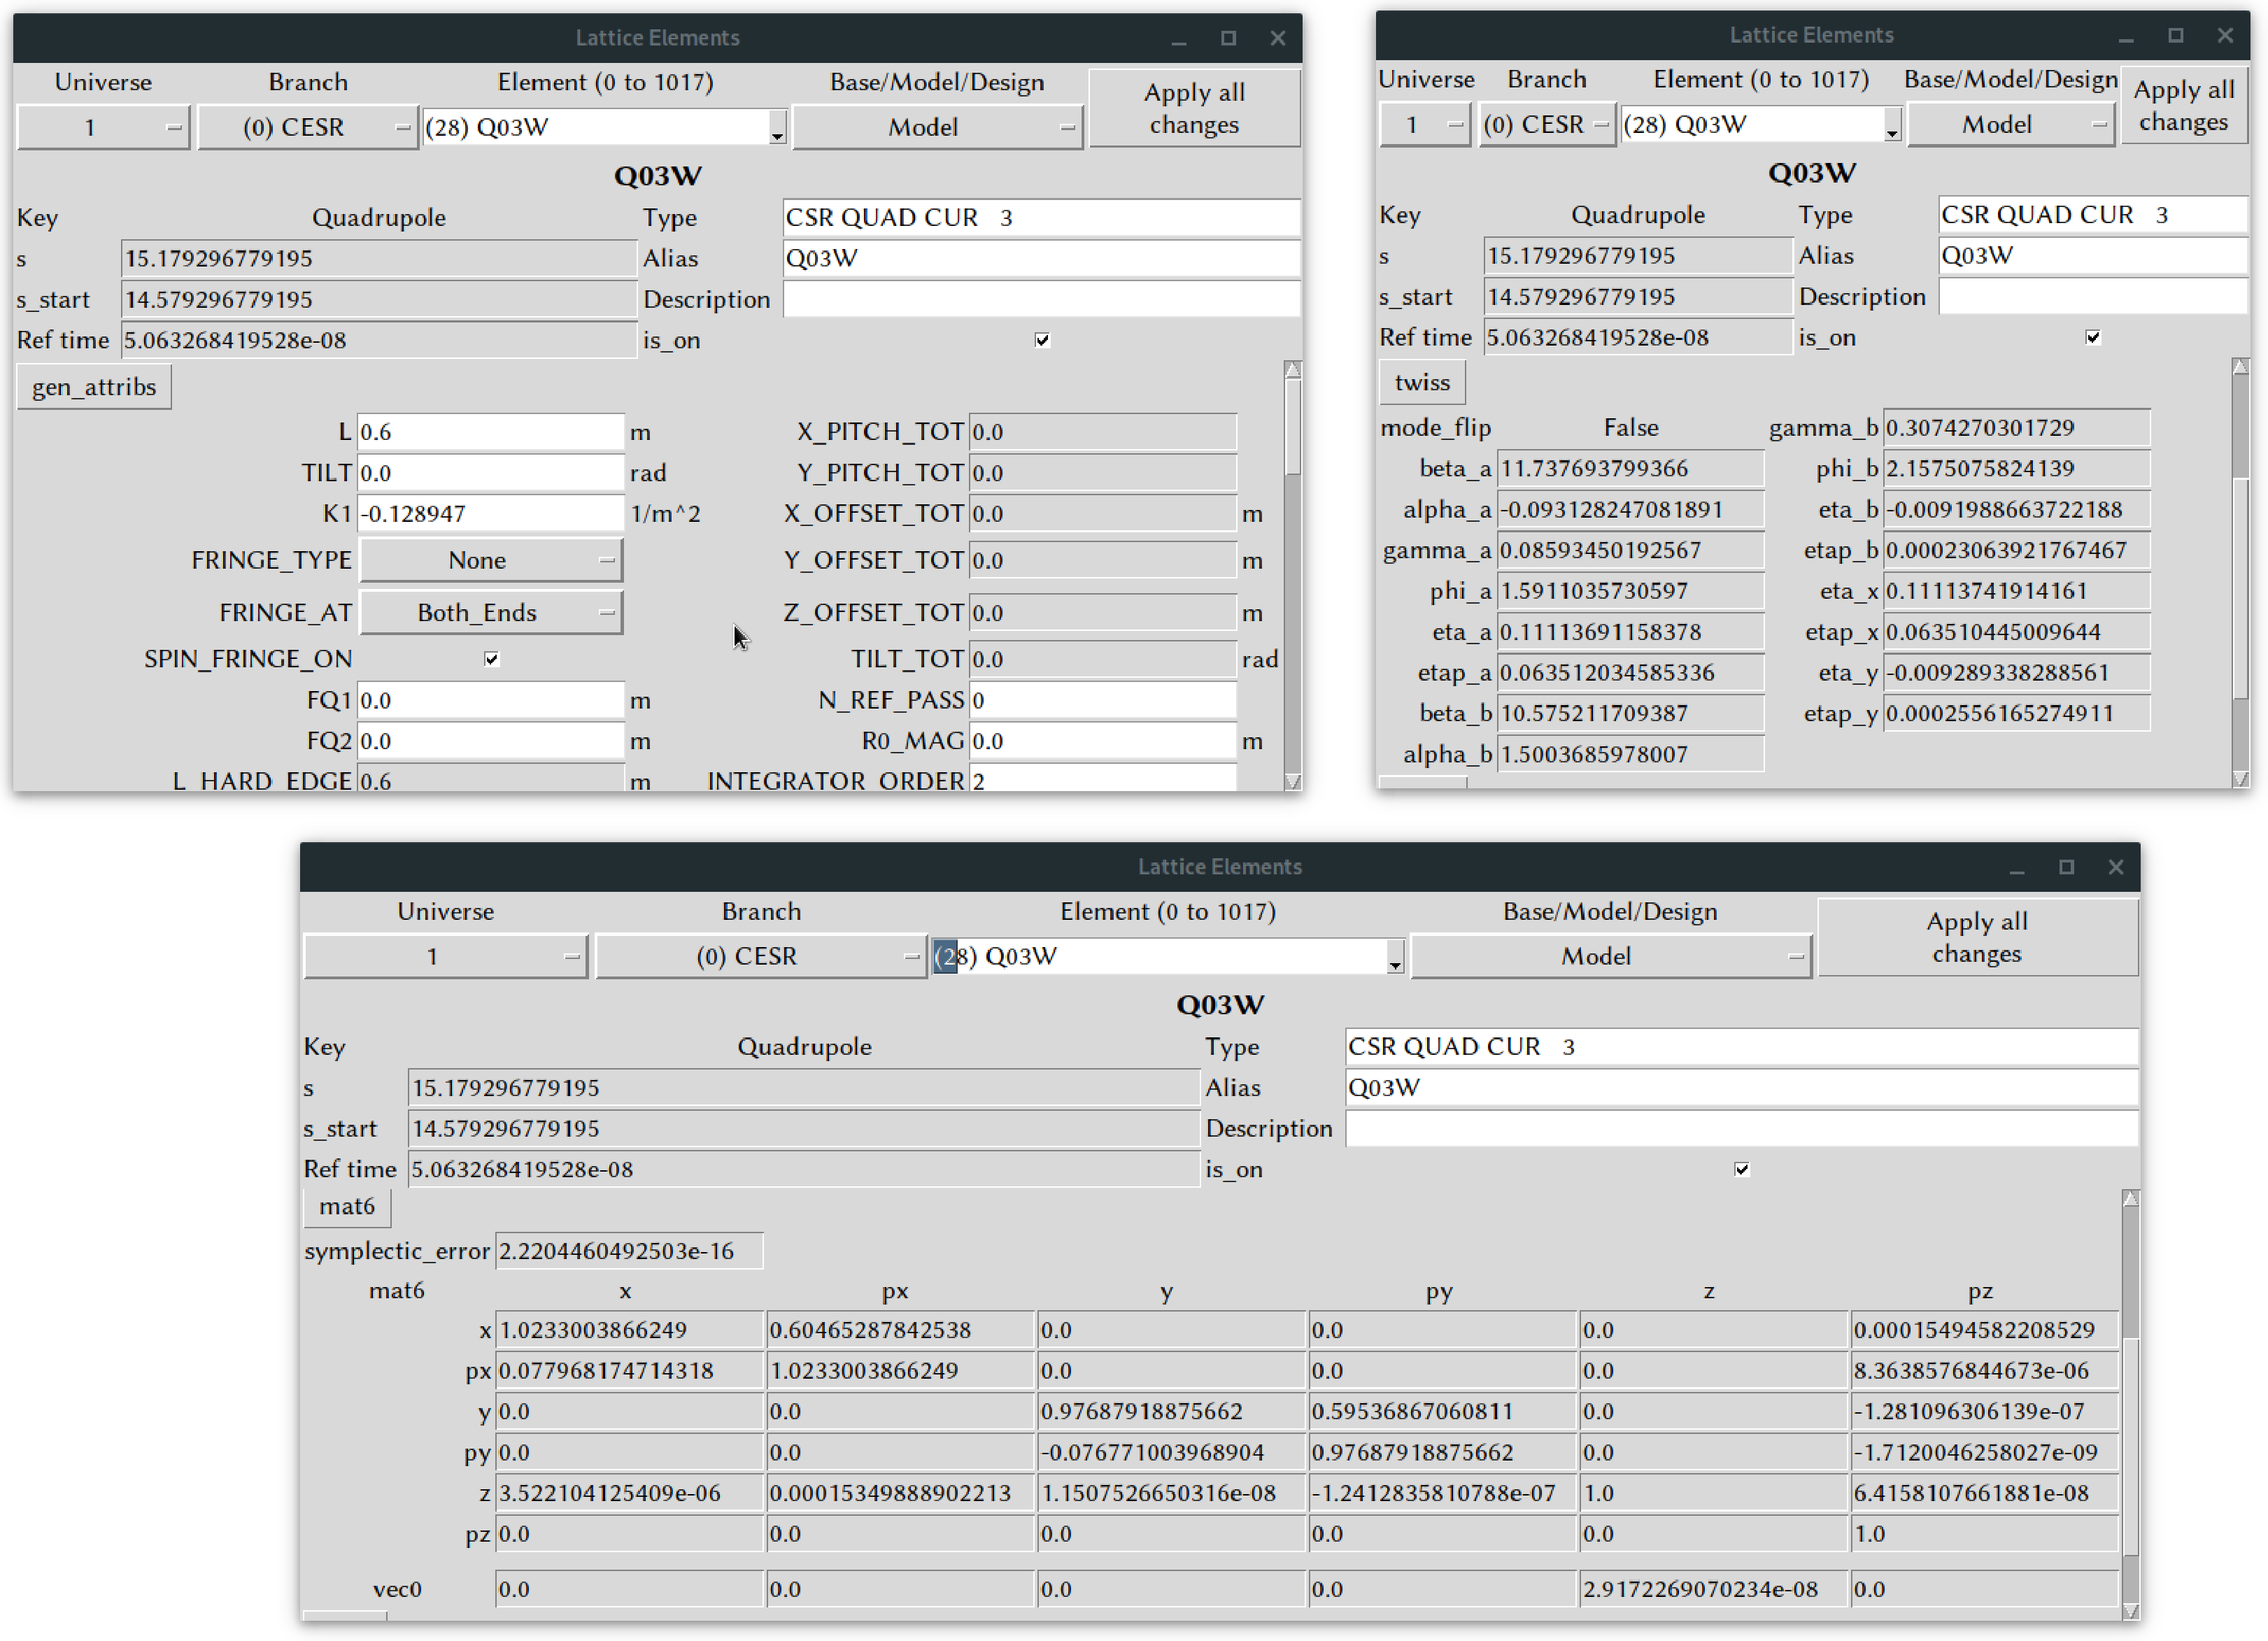
\includegraphics[width=12cm]{figures/lat_element_2.pdf}
\caption[Some of the collapsable sections of the lattice element window.]{Some of the collapsable sections of the lattice element window.
Top left: the gen_attribs section.
Top right: the twiss section.
Bottom: the mat6 section.}
\label{fig:gui.lat.element.2}
\end{figure}
Most of the sections display properties in text boxes or drop down menus, some of which can be editted.
There are a few key exceptions to this rule that are listed below.

\begin{figure}
\centering
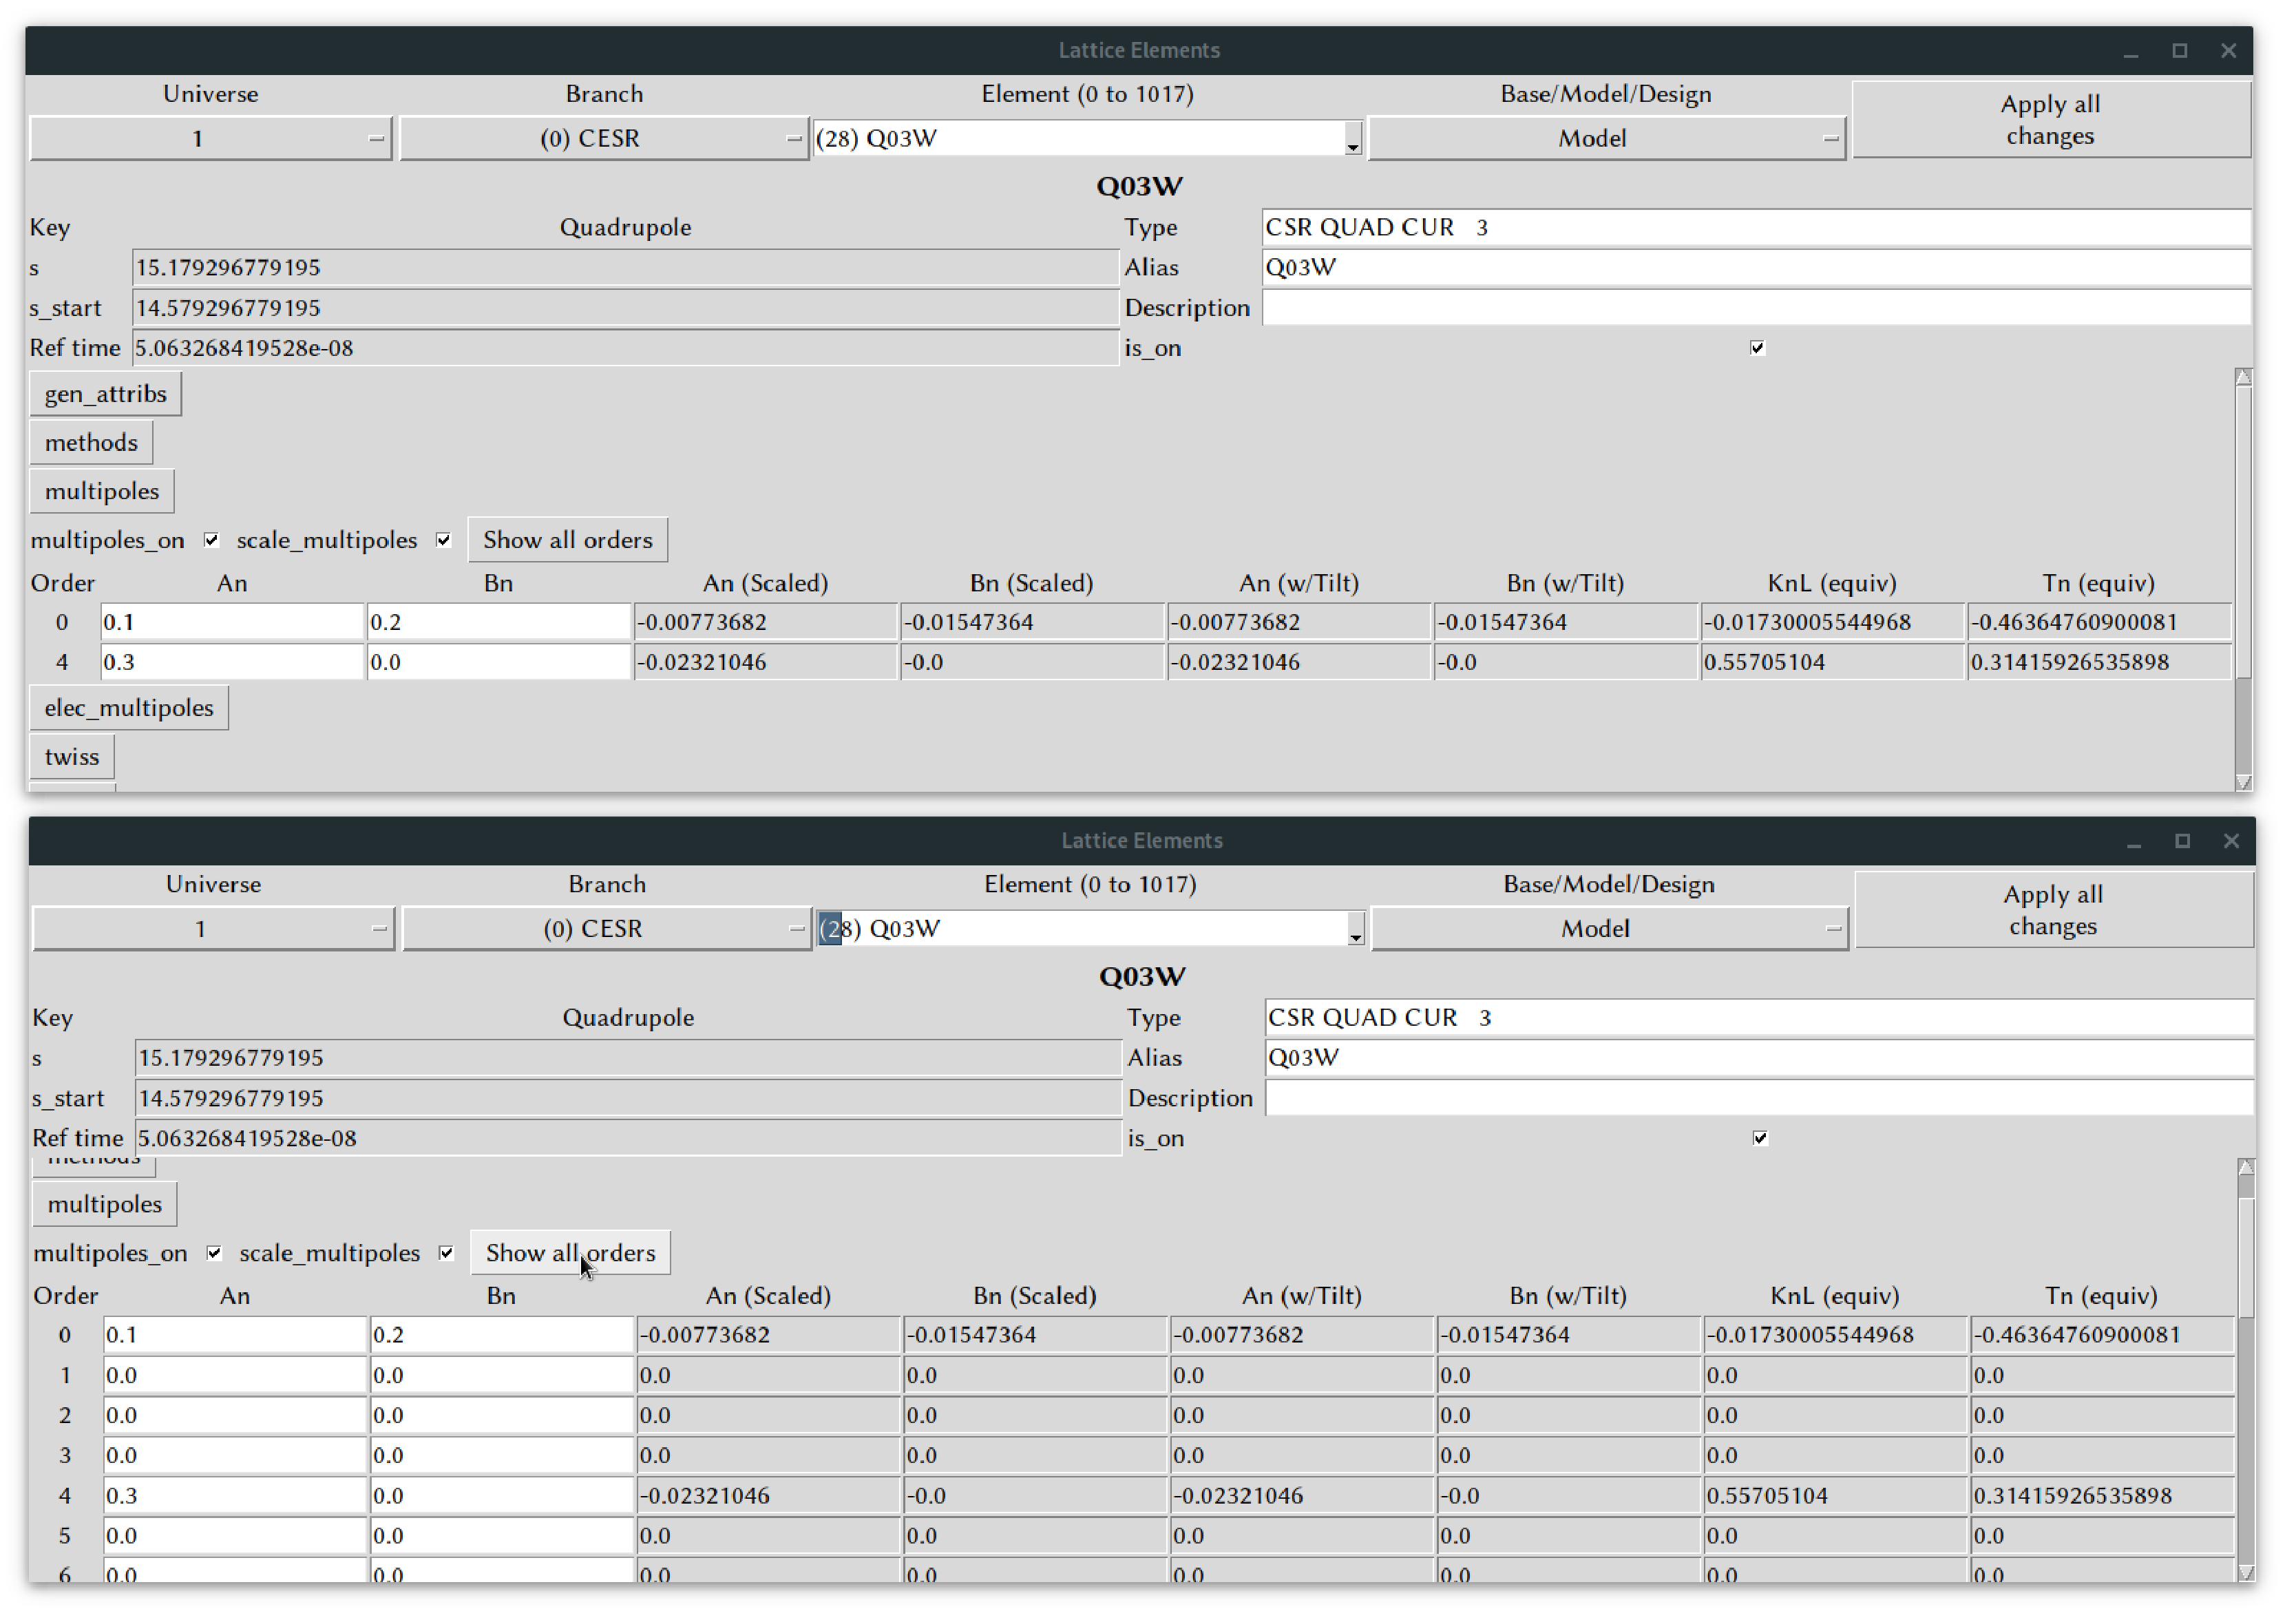
\includegraphics[width=10cm]{figures/lat_element_multipoles.pdf}
\caption[The magnetic multipoles for Q03W.]{The magnetic multipoles for Q03W.
Top: by default, only the nonzero multipoles are shown in the table.
Bottom: clicking on the "Show all orders" button will expand the table to allow the user to edit any of the element's multipoles.}
\label{fig:gui.lat.element.multipoles}
\end{figure}
Elements that have multipoles and/or electric multipoles will have their multipole values displayed in a table under the respective section.
This is shown in Figure \ref{fig:gui.lat.element.multipoles}
By default, only the orders for which the the multipole is nonzero are shown.
Clicking th3e "Show all orders" button will expand the table to show all multipole orders.
The user can then set the multipole strengths of any order as desired.

\begin{figure}
\centering
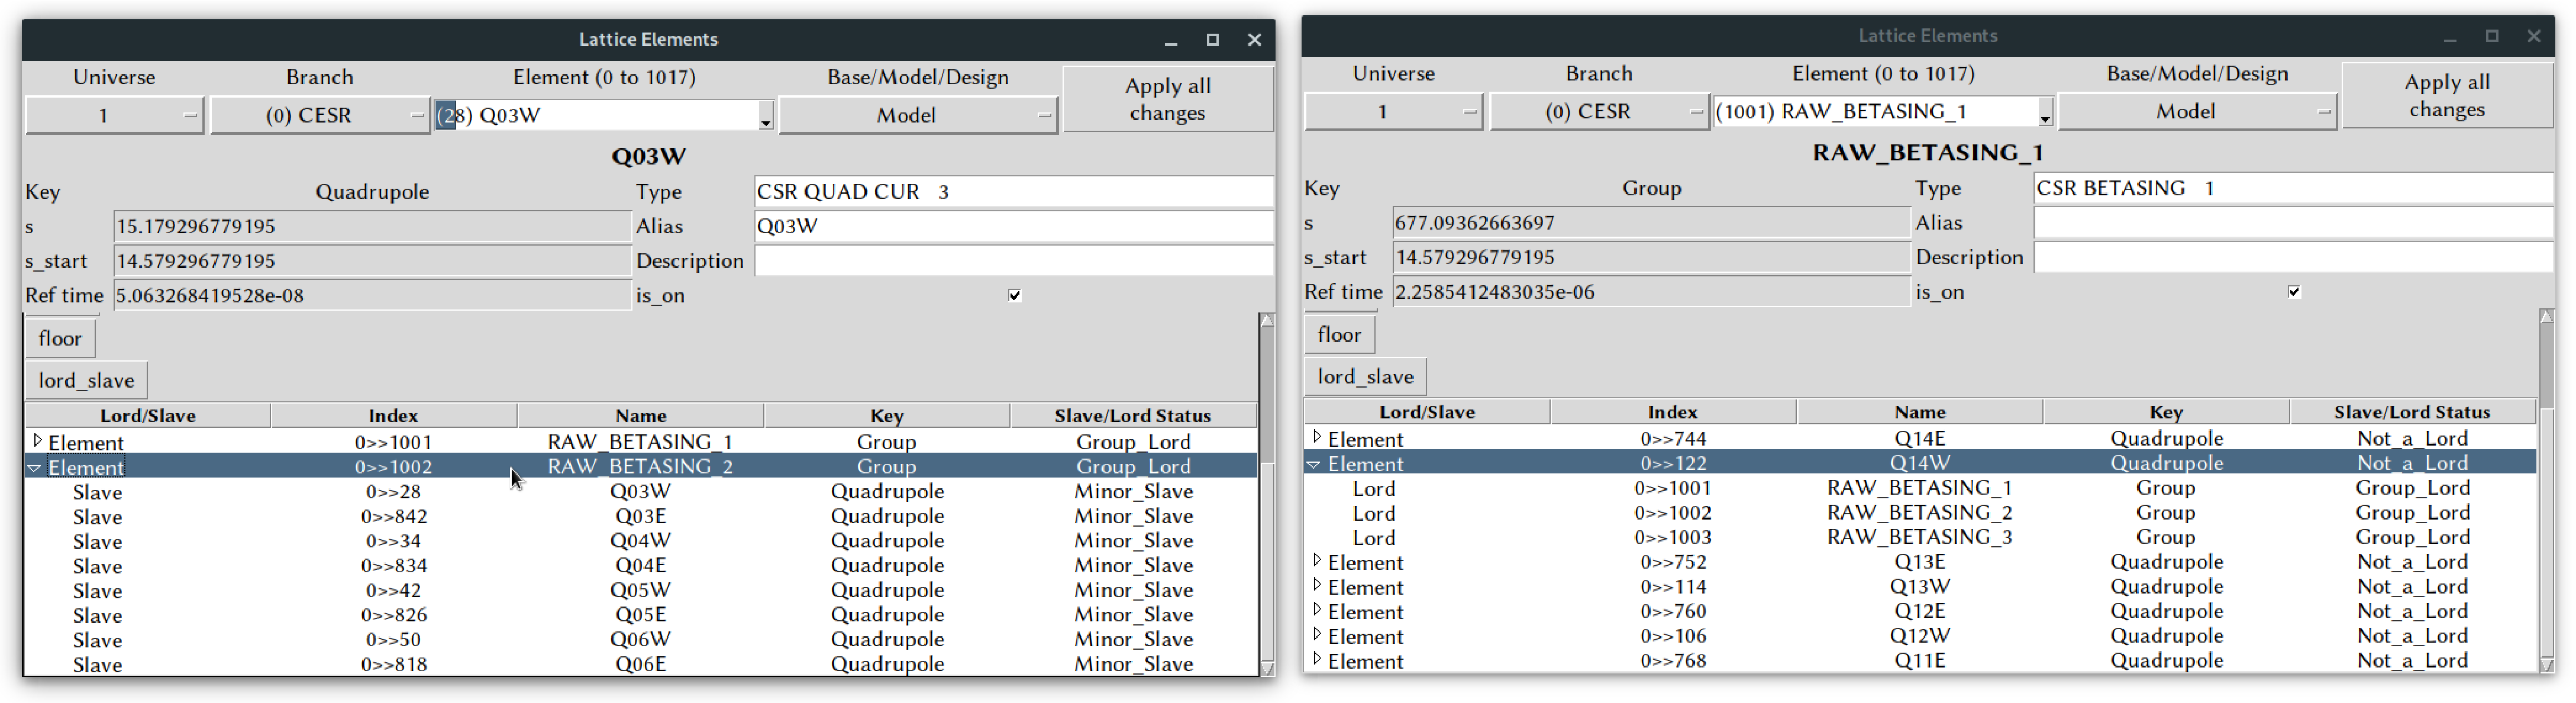
\includegraphics[width=12cm]{figures/lat_lord_slave.pdf}
\caption[The lord_slave section of the lattice element window.]{The lord_slave section of the lattice element window.
Left: Q03W is a slave element, and its lords are listed in the table.
One of the lords, RAW_BETASING_2, is expanded to show its slaves.
Right: RAW_BETASING_1 is a lord element, and its slaves are listed in the table.
One of the slaves, Q14W, is expanded to show its lords.}
\label{fig:gui.lat.element.lordslave}
\end{figure}

The other important exception is the lord_slave section, which displays an element's associated lords and slaves.
For elements that are slaves, this section will list the element's lords in a table.
Clicking on the arrow next to a lord's name will expand a list of that lord's slaves.
Likewise, for a lord element, this section displays a list of the element's slaves.
Clicking on the arrow next to one of these slaves will expand a list of that element's lords.
As with the lattice table, double clicking on an element in the lord/slave list will open another element window for that element.
This is illustrated in Figure \ref{fig:gui.lat.element.lordslave}.
Once the information in each section has been modified as needed, clicking the "Apply all changes" button will change the element properties in Tao.
